\section{Monoidal objects in locally cubical bicategories}
\label{sec:mono-objects}

We now move on to define an appropriate abstract sort of ``monoidal object'' that will be preserved by the product-preserving functor $\cH$, and that specializes to monoidal double categories and to monoidal bicategories.
It would be nice if we could stay entirely in the world of iconic tricategories (that is, \Icon-enriched bicategories); but unfortunately the usual composition of monoidal functors between monoidal bicategories is not strictly associative, so they do not form an iconic tricategory.

However, they do form a more general structure, namely a bicategory enriched over \cDbl; in~\cite{gg:ldstr-tricat} this is called a \textbf{locally cubical bicategory}.
Since any bicategory can be regarded as a double category with only identity 1-morphisms, any iconic tricategory can be regarded as a locally cubical bicategory, but the latter are more general.
In particular, in a locally cubical bicategory the composition of 1-morphisms is associative only up to an invertible (vertical) 2-morphism.
And indeed, one of the results of~\cite{gg:ldstr-tricat} is that monoidal bicategories form a locally cubical bicategory; here we will generalize this to monoidal objects, perhaps braided and symmetric, in any iconic tricategory with finite products --- and indeed, in any locally cubical bicategory with finite products.

Since \cDbl\ is also a cartesian monoidal 2-category, we can define what it means for a locally cubical bicategory to have finite products, and this property is preserved when regarding an iconic tricategory as a locally cubical bicategory.
In particular, this applies to \cDblf\ and to \cBicat\ --- but actually, in place of the iconic tricategory \cBicat\ considered up until now we will focus instead on the locally cubical bicategory of bicategories constructed in~\cite{gg:ldstr-tricat}, whose ``locally horizontal part'' is \cBicat, but whose vertical 2-cells are \emph{icons}.
We denote this by \fBicat; it is easy to see that it also has products preserved by the inclusion $\cBicat\to \fBicat$, so that the composite functor $\cH : \cDblf \to\fBicat$ still preserves products.

We now define symmetric, braided and monoidal structures on objects, 1-cells, 2-cells, and 3-cells internal to a locally cubical bicategory with products, by taking the definitions of monoidal, braided, and symmetric structure for bicategories given in~\cite{nick:tricatsbook},~\cite{mccrudden:bal-coalgb}, and~\cite{gg:ldstr-tricat} and regarding the data of bicategories, functors, pseudonatural transformations, and modifications abstractly as objects, 1-cells, 2-cells, and 3-cells in a locally cubical bicategory.

Note that under this translation pseudonatural transformations become \emph{horizontal} 2-cells and modifications become globular 3-cells.
The horizontal 2-cells in \cDblf\ (which has no nonidentity vertical 2-morphisms) are the (vertical) transformations, while those in \fBicat\ are exactly the pseudonatural transformations (its vertical 2-morphisms are icons).
Let \fB\ be a locally cubical bicategory with products.

Locally cubical bicategories have three types of composition. Firstly, composition of 1-cells, 2-cells, and 3-cells along a 0-cell boundary, which we will denote with "$\comp$". We will often omit it, when it is clear from the context and just write the juxtaposition of 1-cells. This composition is weak with weak identities. We write $\compI$ for the unit double category, and $\compa, \compr$, and $\compl$ for the associator and unitors. Secondly, we have horizontal composition of horizontal 2-cells along a 1-cell boundary and horizontal composition of 3-cells along a vertical 2-cell bounday, which we will denote with "$\horc$". This composition is weakly associative and horizontal identities hold up to isomorphism. We write $U_{\alpha}$ for the horizontal identity on a 2-cell 
$\alpha$ and we denote the structure maps related to associativity and units as $\hora, \horr$, $\horl$.
Thirdly, vertical composition of vertical 2-cells along a 1-cell boundary and vertical composition of 3-cells along a horizontal 2-cell boundary, which we will denote with "$\verc$". This composition is strictly associative and has strict identities.

\begin{defn}
A {\bf monoidal object} in \fB\ is an object $A$, equipped with 1-cells $\otimes_A: A \times A \rightarrow A$ and $I_A: * \rightarrow A$, and horizontal 2-cells
\begin{itemize} 
\item $\alpha: \ten  (\id \times \tens) \xslashedRightarrow{} \ten (\tens \times \id)$
\item $l: \ten (I \times \id) \xslashedRightarrow{} \id$ and $r:\ten (\id \times I) \xslashedRightarrow{} \id$ 
\end{itemize}
Finally, it must be equipped with the invertible globular 3-cells $\pi, \mu, \lambda, \rho$, relating the two different ways around the Mac Lane pentagon and the three other coherence diagrams given in Definition 4.1 of~\cite{nick:tricatsbook}, which satisfy the appropriate three axioms.

A monoidal object is {\bf braided} if in addition there is a horizontal 2-cell $\sigma_A: \tens \xslashedRightarrow{} \ten \tau$, where $\tau: A \times A \rightarrow A \times A$ interchanges the two copies of $A$; and if there are invertible globular 3-cells 

\begin{equation}
  \begin{aligned}
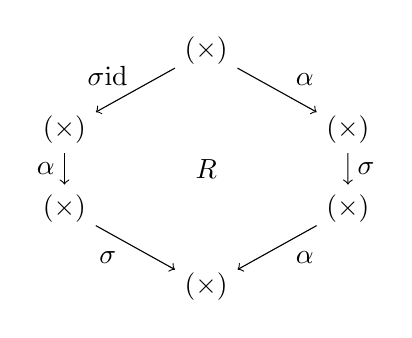
\begin{tikzpicture}[xscale=0.9]
\node (t) at (2,3) {$\ten (\ten \times \id)$};
\node (tl) at (0,2) {$\ten(\ten \times \id)$};
\node (bl) at (0,1) {$\ten (\id \times \ten)$};
\node (b) at (2,0) {$\ten (\id \times \ten)$};
\node (tr) at (4,2) {$\ten(\id \times \ten)$};
\node (br) at (4,1) {$\ten (\ten \times \id)$};
\draw[->] (t) to node [above,xshift=10pt, yshift=-2] {$\alpha$} (tr);
\draw[->] (tr) to node [right] {$\sigma$} (br);
\draw[->] (br) to node [below,xshift=10pt, yshift=2pt] {$\alpha$} (b);
\draw[->] (t) to node [above,xshift=-10pt, yshift=-2pt] {$\sigma \ten \mbox{id}$} (tl);
\draw[->] (tl) to node [left] {$\alpha$} (bl);
\draw[->] (bl) to node [below,xshift=-10pt,yshift=2pt] {$\mathid \ten \sigma$} (b);
\node at (2,1.5) {$\DDownarrow R \iso$};
\end{tikzpicture}
  \end{aligned}
\hspace{5pt}\mbox{and} \hspace{5pt}
\begin{aligned}
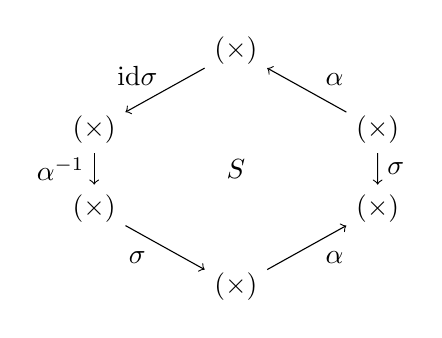
\begin{tikzpicture}[xscale=0.9]
\node (t) at (2,3) {$\ten(\id \times \ten)$};
\node (tl) at (0,2) {$\ten(\id \times \ten)$};
\node (bl) at (0,1) {$\ten(\ten \times \id)$};
\node (b) at (2,0) {$\ten(\ten \times \id)$};
\node (tr) at (4,2) {$\ten(\ten \times \id)$};
\node (br) at (4,1) {$\ten(\id \times \ten)$};
\draw[->] (tr) to node [above,xshift=10pt, yshift=-2] {$\alpha$} (t);
\draw[->] (tr) to node [right] {$\sigma$} (br);
\draw[->] (b) to node [below,xshift=10pt, yshift=2pt] {$\alpha$} (br);
\draw[->] (t) to node [above,xshift=-10pt, yshift=-2pt] {$\mbox{id} \ten \sigma$} (tl);
\draw[->] (tl) to node [left] {${\alpha}^{-1}$} (bl);
\draw[->] (bl) to node [below,xshift=-10pt,yshift=2pt] {$\sigma \ten \mathid$} (b);
\node at (2,1.5) {$\DDownarrow S \iso$};
\end{tikzpicture}
\end{aligned}
\end{equation}
satisfying the axioms (BA1), (BA2), (BA3), and (BA4) given in~\cite[p136--139]{mccrudden:bal-coalgb} . 
It is {\bf sylleptic} when there exists an invertible globular 3-cell

 \[
 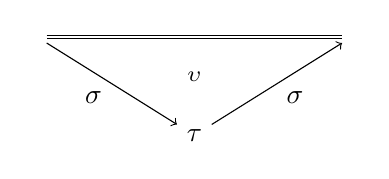
\begin{tikzpicture}
 \node (tl) at (-2,1) {$\ten$};
 \node (tr) at (2,1) {$\ten$};
 \node (b) at (0,-.25) {$\tens \tau$};
 \draw[double] (tl)  -- (tr);
 \draw[->] (tl) to node[left, yshift=-5pt]{$\sigma$} (b);
 \draw[->] (b) to node[right, yshift=-5pt] {$\sigma$}(tr);
 \node at (0,0.5) {\footnotesize $\DDownarrow \upsilon \iso$}; 
 \end{tikzpicture}
 \]
  satisfying the axioms (SA1), (SA2) on~\cite[p144--145]{mccrudden:bal-coalgb}. It is {\bf symmetric} if in addition, it satisfies the axiom given on~\cite[p91]{mccrudden:bal-coalgb}.
\end{defn}

By construction, these definitions give the expected results in \fBicat.
In \cDblf, where there are no nonidentity 3-cells, they reduce to the definitions from section~\ref{sec:symm-mono-double}; and in particular every syllepsis is a symmetry.

\begin{defn}
Let $A,B$ be monoidal objects in \fB. A 1-cell $f:A \rightarrow B$ is {\bf lax monoidal} when it is equipped with the following horizontal 2-cells:
\begin{itemize}
\item $\chi: \ten_B (f \times f) \xslashedRightarrow{} f  \otimes_A$
\item $\iota: I_B \xslashedRightarrow{} f I_A$
\end{itemize}
As well as globular invertible 3-cells $\omega: \alpha_A \horc \chi \horc (\chi \times \id) \RRightarrow \chi \horc (\id \times \chi) \horc \alpha_B$ , $\gamma: (\id \times l) \horc \chi \horc (\iota \times \id) \RRightarrow l$, and $\delta: (
id \odot l) \horc \chi \horc (\id \times \iota) \RRightarrow r$ given in Definition 4.10 of~\cite{nick:tricatsbook}, expressing the usual associativity and unitality conditions, which satisfy the two given commutativity axioms.
A monoidal 1-cell is called {\bf braided}, when $A$ and $B$ are braided and there is a horizontal 2-cell $u: \sigma_B \horc \chi  \xslashedRightarrow \chi \horc (f \sigma_A)$, satisfying the braiding axioms analogous to (BHA1) and (BHA2) given in  \cite[p141-142]{mccrudden:bal-coalgb}. It is {\bf symmetric} when $A$ and $B$ are symmetric and the 3-cells defining the braided monoidal structure of $f$ satisfy the additional axiom analogous to  (SHA1) given in   \cite[p145]{mccrudden:bal-coalgb}.

When the natural transformations are in the opposite direction, the functor is {\bf oplax monoidal}, and when they are isomorphisms, the functor is {\bf strong monoidal}.
\end{defn}



\begin{defn}\label{Def:monverttrans}
Let $f, g:A \rightarrow B$ be lax monoidal 1-cells in \fB. A {\bf lax monoidal 2-cell} $\alpha: f \xslashedRightarrow{} g$ is a horizontal 2-cell in \fB\ that is equipped with globular 3-cells
\begin{itemize}
\item $\Pi: \chi_f \horc (\alpha \comp U_{\ten}) \xslashedRightarrow{} U_{\ten}(\alpha, \alpha) \horc \chi_g$
\item $M: \iota_f \horc (\alpha \comp U_{\ten}) \xslashedRightarrow{} \iota_g$
\end{itemize}

Such that coherence equations analogous to (IA1)-(IA3) of~\cite{gg:ldstr-tricat} hold.
An {\bf oplax monoidal 2-cell} between oplax monoidal 1-cells, is a 2-cell with the same data, but with the arrows in the opposite direction. If $g,f$ are strong monoidal and $\Pi, M$ are isomorphisms, we call $\alpha$ a {\bf strong monoidal 2-cell}.
such that the three coherence axioms in definition 3 of~\cite{gg:ldstr-tricat} hold.
A monoidal 2-cell is {\bf braided} or {\bf symmetric} when $f,g$ are braided or symmetric, and in addition the coherence axiom analogous to (BTA1) of~\cite[p143]{mccrudden:bal-coalgb} holds. Note that here the author writes $\rho$ for our braiding 1-cell $\sigma$.
\end{defn}

As remarked above, we will actually construct a locally cubical bicategory of monoidal objects.
The monoidal 2-cells will be the horizontal 2-cells therein; we now define the vertical 2-morphisms.

\begin{defn}\label{Def:monicon}
  Let $f, g:A \rightarrow B$ be lax monoidal 1-cells in \fB.
  A \textbf{lax monoidal icon} $\alpha: f \Rightarrow g$ is a (vertical) 2-morphism in \fB\ that is equipped with 3-cells
\begin{equation}
\begin{aligned}
 \begin{tikzpicture}[scale=2]
 \node (tl) at (0,1) {$I_B$};
 \node (tr) at (1,1) {$f I_A$};
 \node (bl) at (0,0) {$I_B$};
 \node (br) at (01,0) {$g I_A$}; 
 \draw[doubletick] (tl)  to node[above]{$\iota_f$} (tr);
 \draw[doubleeq] (tl) to (bl);
 \draw[doubletick] (bl) to node[below] {$\iota_g$}(br);
  \draw[darrow] (tr) to node[right] {$\alpha \comp \id_I$}(br);
 \node at (0.5,0.5) {\footnotesize $\DDownarrow M^{\alpha}$}; 
 \end{tikzpicture}
 \end{aligned}
 \hspace{.5cm}
 \begin{aligned}
  \begin{tikzpicture}[scale=2]
 \node (tl) at (0,1) {$\ten (f \times f)$};
 \node (tr) at (1,1) {$f \ten$};
 \node (bl) at (0,0) {$\ten(g \times g)$};
 \node (br) at (01,0) {$g  \ten$}; 
 \draw[doubletick] (tl)  to node[above]{$\chi_f$} (tr);
 \draw[doubleeq] (tl) to node[left]{$\id_{\ten} (\alpha \times \alpha)$} (bl);
 \draw[doubletick] (bl) to node[below] {$\chi_g$}(br);
  \draw[darrow] (tr) to node[right] {$\alpha \comp \id_{\ten}$}(br);
 \node at (0.5,0.5) {\footnotesize $\DDownarrow \Pi^{\alpha}$}; 
 \end{tikzpicture}
\end{aligned}
\end{equation}

such that the coherence axioms (TA2), (TA3), and (TA4) analogous to definition 2 of~\cite{gg:ldstr-tricat} hold.
An {\bf oplax monoidal icon} between oplax monoidal 1-cells, is a 2-cell with the same data. If $g,f$ are strong monoidal and $\Pi, M$ are isomorphisms, we call $\alpha$ a {\bf strong monoidal icon}.
A monoidal icon is {\bf braided} or {\bf symmetric} when $f,g$ are braided or symmetric, and in addition the coherence axiom analogous to (BTA1) of~\cite[p143]{mccrudden:bal-coalgb} holds. Note that here the author writes $\rho$ for our braiding 1-cell $\sigma$.
\end{defn}

\begin{defn}
  Let $f,g,f',g' A \rightarrow B$ be monoidal 1-cells, let $\alpha: f \xslashedRightarrow{} g$, $\beta: f' \xslashedRightarrow{} g'$ be monoidal 2-cells, and let $\gamma: f \Rightarrow f'$, $\delta: g \Rightarrow g'$ be monoidal icons. A \textbf{monoidal 3-cell} is a 3-cell 
  
   \[
 \begin{tikzpicture}[scale=2]
 \node (tl) at (0,1) {$f$};
 \node (tr) at (1,1) {$g$};
 \node (bl) at (0,0) {$f'$};
 \node (br) at (01,0) {$g'$}; 
 \draw[doubletick] (tl)  to node[above]{$\alpha$} (tr);
 \draw[darrow] (tl) to node[left]{$\gamma$} (bl);
 \draw[doubletick] (bl) to node[below] {$\beta$}(br);
  \draw[darrow] (tr) to node[right] {$\delta$}(br);
 \node at (0.5,0.5) {\footnotesize $\DDownarrow \Gamma$}; 
 \end{tikzpicture}
 \]
 
 Such that the two equalities below hold.
 
 \begin{equation}
\begin{aligned}
 \begin{tikzpicture}[scale=2]
 \node (tl) at (0,1) {$f  I_A$};
 \node (tr) at (1,1) {$g  I_A$};
 \node (bl) at (0,0) {$f' I_A$};
 \node (br) at (01,0) {$g' I_A$}; 
 \draw[doubletick] (tl)  to node[above]{$\alpha \comp U_I$} (tr);
 \draw[darrow] (tl) to node[left]{$\gamma \comp \id_I$} (bl);
 \draw[doubletick] (bl) to node[above] {$\beta \comp U_I$}(br);
  \draw[-implies, double equal sign distance] (tr) to node[right] {$\delta \comp \id_I$}(br);
 \node at (0.5,0.5) {\footnotesize $\DDownarrow \Gamma \comp \id$}; 
 \node (tl1) at (-1,0) {$I_B$};
 \node (bl1) at (-1,-1) {$I_B$};
 \draw[doubletick] (tl1)  to node[above]{$\iota^f$} (tl);
 \draw[doubleeq] (tl1) to (bl1);
 \draw[doubletick] (bl1) to node[above]{$\iota^{f'}$}(bl);
 \node at (-0.5,0) {\footnotesize $\DDownarrow M^{\gamma}$};
  \node (br1) at (0,-1) {$I_B$};
 \draw[doubleeq] (bl1)  to (br1);
 \draw[doubletick] (br1) to  node[right]{$\iota^{g'}$}(br);
 \node at (0,-0.5) {\footnotesize $\DDownarrow M^{\beta}$}; 
 \end{tikzpicture}
\end{aligned}
 =
 \begin{aligned}
  \begin{tikzpicture}[scale=2]
 \node (tl) at (0,1) {$I_B$};
 \node (tr) at (1,1) {$I_B$};
 \node (bl) at (0,0) {$I_B$};
 \node (br) at (01,0) {$I_B$}; 
 \draw[doubleeq] (tl)  to (tr);
 \draw[doubleeq] (tl) to  (bl);
 \draw[doubleeq] (bl) to (br);
 \draw[doubleeq] (tr) to (br);
 \node at (0.5,0.5) {\footnotesize $=$}; 
 \node (tl1) at (1,2) {$f I_A$};
 \node (tr1) at (2,2) {$g I_A$};
 \draw[doubletick] (tl)  to node[above]{$\iota^f$} (tl1);
 \draw[doubletick] (tl1) to node[above]{$\alpha \comp U_I$} (tr1);
 \draw[doubletick] (tr) to node[above]{$\iota^{g}$}(tr1);
 \node at (1,1.5) {\footnotesize $\DDownarrow M^{\alpha}$};
  \node (br1) at (2,1) {$g' I$};
 \draw[doubletick] (br)  to node[below]{$\iota^{g'}$} (br1);
 \draw[darrow] (tr1) to  node[right]{$\delta \comp \id_I$}(br1);
 \node at (1.5,1) {\footnotesize $\DDownarrow M^{\delta}$}; 
 \end{tikzpicture}
 \end{aligned}
\end{equation}

 \begin{equation}
\begin{aligned}
 \begin{tikzpicture}[scale=2]
 \node (tl) at (0,1) {$f\ten$};
 \node (tr) at (1,1) {$g \ten$};
 \node (bl) at (0,0) {$f' \ten$};
 \node (br) at (01,0) {$g' \ten$}; 
 \draw[doubletick] (tl)  to node[above]{$\alpha \comp U_{\ten}$} (tr);
 \draw[darrow] (tl) to node[left]{$\gamma \comp U_{\ten}$} (bl);
 \draw[doubletick] (bl) to node[above, xshift=1pt, yshift=-1pt] {$\beta \comp \id_{\ten}$}(br);
  \draw[darrow] (tr) to node[right] {$\delta \comp \id_{\ten}$}(br);
 \node at (0.5,0.5) {\footnotesize $\DDownarrow \Gamma \comp \id$}; 
 \node (tl1) at (-1,0) {$\ten  (f\times f)$};
 \node (bl1) at (-1,-1) {$\ten  (f'\times f')$};
 \draw[doubletick] (tl1)  to node[above]{$\chi^f$} (tl);
 \draw[darrow] (tl1) to node[left]{$\id_{\ten} (\gamma \times \gamma)$} (bl1);
 \draw[doubletick] (bl1) to node[above]{$\chi^{f'}$}(bl);
 \node at (-0.5,0) {\footnotesize $\DDownarrow \Pi^{\gamma}$};
  \node (br1) at (0,-1) {$\ten (g'\times g')$};
 \draw[doubleeq] (bl1)  to node[below]{$\id_{\ten} (\beta \times \beta)$} (br1);
 \draw[doubletick] (br1) to  node[right]{$\chi^{g'}$}(br);
 \node at (0,-0.5) {\footnotesize $\DDownarrow \Pi^{\beta}$}; 
 \end{tikzpicture}
\end{aligned}
 =
 \begin{aligned}
  \begin{tikzpicture}[yscale=2, xscale=2.5]
 \node (tl) at (0,1) {$\ten (f\times f)$};
 \node (tr) at (1,1) {$\ten (g\times g)$};
 \node (bl) at (0,0) {$\ten (f'\times f')$};
 \node (br) at (01,0) {$\ten (g'\times g')$}; 
 \draw[doubletick] (tl)  to node[below]{$U_{\ten} (\alpha \times \alpha)$} (tr);
 \draw[darrow] (tl) to node[left]{$\id_{\ten} (\gamma \times \gamma)$}  (bl);
 \draw[doubletick] (bl) to node [below] {$U_{\ten} (\beta \times \beta)$} (br);
  \draw[darrow] (tr) to node[right,yshift=5pt]{$\id_{\ten} (\delta \times \delta)$} (br);
 \node at (0.5,0.5) {\footnotesize $\DDownarrow \id \comp (\Gamma \times \Gamma)$}; 
 \node (tl1) at (1,2) {$f \ten$};
 \node (tr1) at (2,2) {$g \ten$};
 \draw[doubletick] (tl)  to node[above]{$\chi^f$} (tl1);
 \draw[doubletick] (tl1) to node[above]{$\alpha \comp U_{\ten}$} (tr1);
 \draw[doubletick] (tr) to node[above]{$\chi^{g}$}(tr1);
 \node at (1,1.5) {\footnotesize $\DDownarrow \Pi^{\alpha}$};
  \node (br1) at (2,1) {$g' \ten$};
 \draw[doubletick] (br)  to node[below]{$\chi^{g'}$} (br1);
 \draw[darrow] (tr1) to  node[right]{$\delta \comp \id_{\ten}$}(br1);
 \node at (1.5,1) {\footnotesize $\DDownarrow \Pi^{\delta}$}; 
 \end{tikzpicture}
 \end{aligned}
\end{equation}
 
\end{defn}

\begin{thm}\label{thm:lcbc}
  Monoidal objects, lax monoidal 1-cells, monoidal 2-cells, monoidal icons, and monoidal 3-cells in \fB\ form a locally cubical bicategory $\cM on\cB$. The same statement holds for colax and strong monoidal objects and cells and for braided, sylleptic, and symmetric objects and cells.
\end{thm}

\begin{proof}
The first step in this proof is to show that for every two monoidal objects $A,B$, the lax monoidal 1-cells, 2-cells and 3-cells in $\cB(A,B)$ form a double category. Likewise for the oplax and strong monoidal cells and for the braided and for the symmetric cells.

First of all, lax monoidal 1-cells and icons form a category.  For each monoidal 1-cell $f:A \rightarrow B$, the identity on $f$ is given by the identity 2-cell $\id_f$, together with the following 3-cells $M^{\id_f} := \id_{\iota_f}$ and $\Pi^{\id_f} := \id_{\chi_f}$. Note that $\comp$ preserves identities strictly, so this is well-defined. The conditions for monoidal 3-cells are trivially satisfied.  For each two monoidal 1-cells $f,g$ and monoidal icons $\alpha, \beta: f \Rightarrow g$, the composite vertical 2-cell $\beta \circ \alpha$ can be equiped with the monoidal structure given by the composites $M^{\beta \circ \alpha} := M^{\beta} \circ M^{\alpha}$ and $\Pi^{\beta\circ \alpha} : = \Pi^{\beta} \circ \Pi^{\alpha}$.  We have a strict interchange law between $\verc$ and $\comp$, so these 3-cells are well-defined. The coherence conditions (TA1)-(TA4) hold by componentwise application of the coherence equalities for $M^{\beta \verc \alpha}$ and $\Pi^{\beta \verc \alpha}$. The same argument holds for oplax and strong monoidal 1-cells and icons.

Furthermore, lax monoidal 2-cells and monoidal 3-cells form a category. For every lax monoidal 2-cell $\alpha: f \xslashedRightarrow{} g$, the identity 3-cell $\id_{\alpha}$ in $\cB$  is monoidal, since the required two equations are trivially satisfied.
For any two monoidal 3-cells $N: \alpha \Rightthreecell \beta$, $K:\beta \Rightthreecell \gamma$, the composition $K \circ N$ in $\cB$ is a monoidal 3-cell. The equations for monoidal 3-cells hold as these are composites of the equations for $N$ and $K$. The same is true for oplax and strong monoidal 2-cells.

Now we describe the horizontal structure.
Let $\alpha:f \xslashedRightarrow{} g$ and $\beta: g \xslashedRightarrow{} h$ be two monoidal 2-cells. Their composition $\alpha \horc \beta$ is monoidal with the following structure 3-cells.

\begin{equation}
M^{\alpha \horc \beta} := 
\begin{aligned}
 \begin{tikzpicture}[yscale=1.5, xscale=3]
 \node (tl) at (0,1) {$I_B$};
\node (tr) at (1,1) {$g   I_A$};
 \node (tm) at (.5,1) {$f  I_A$};
 \node (bl) at (0,0) {$I_B$};
 \node (br) at (1,0) {$g I_A$}; 
 \node (trr) at (1.5,1) {$h I_A$};
 \node (brr) at (1.5,0) {$h I_A$};
 \node (bbr) at (1.5,-1) {$hI_A$};
 \node(bbl) at (0,-1) {$I_B$};
    \draw[darrow] (tl) to[in=120, out=60] node[above]{$(\alpha \horc \beta)\comp U_{I}$} (tr);
 \draw[darrow] (brr) to node[right] {} (bbr);
 \draw[doubleeq] (bl) to (bbl);
 \draw[doubleeq] (bbl) to (bbr);
 \draw[darrow] (tr) to node[above]{$\beta \comp U_I$} (trr);
  \draw[darrow] (br) to node[above]{$\beta \comp U_I$}(brr);
  \draw[doubleeq] (trr) to (brr);
 \draw[doubletick] (tl)  to node[above]{$\iota_f$} (tm);
  \draw[doubletick] (tm)  to node[above]{$\alpha \comp U_I$} (tr);
 \draw[doubleeq] (tl) to (bl);
 \draw[doubletick] (bl) to node[below] {$\iota_f$}(br);
  \draw[doubleeq] (tr) to (br);
 \node at (0.5,0.5) {\footnotesize $M^{\alpha} \DDownarrow \iso $}; 
  \node at (0.75,-.5) {\footnotesize $M^{\beta} \DDownarrow \iso $}; 
   \node at (1.25,.5) {\footnotesize $=$}; 
 \end{tikzpicture}
 \end{aligned}
\end{equation}
\begin{equation}
 \Pi^{\alpha \horc \beta}:=
 \begin{aligned}
  \begin{tikzpicture}[yscale=1.5, xscale=5]
 \node (tl) at (0,1) {$\ten  (f \times f)$};
 \node (tr) at (1,1) {$g \ten$};
 \node (bl) at (0,0) {$\ten  (f \times f)$};
 \node (br) at (01,0) {$g \ten$}; 
 \node(tm) at (.5,1) {$f \ten$};
 \node (bm) at (.5,0) {$\ten (g\times g)$};
 \node (trr) at (1.5,1) {$h \ten$};
  \node (brr) at (1.5,0) {$h \ten$};
  \node (bbl) at (0,-1) {$\ten (f \times f)$};
  \node (bbm) at (.5,-1) {$\ten (g \times g)$}; 
  \node (bbr) at (1,-1) {$\ten (h \times h)$};
  \node (bbrr) at (1.5,-1) {$h \ten $};
 \draw[doubletick] (tl)  to node[above]{$\chi_f $} (tm);
  \draw[doubletick] (tm)  to node[above]{$\alpha \comp U_{\ten}$} (tr);
 \draw[darrow] (tl) to node[left]{$U_{\ten} (f \times f)$} (bl);
  \draw[doubletick] (bl) to node[below] {$U_{\ten}\comp (\alpha \times \alpha)$}(bm);
 \draw[doubletick] (bm) to node[below] {$\chi_g$}(br);
  \draw[doubleeq] (tr) to (br); 
 \draw[doubleeq] (trr) to (brr);
 \draw (tr) to node[above]{$\beta \comp U_{\ten}$} (trr);
 \draw (br) to node[above]{$\beta \comp U_{\ten}$} (brr);
 \draw (bbr) to node[above]{$\chi_h$} (bbrr);
 \draw[doubleeq] (bl) to (bbl);
 \draw[doubleeq] (bm) to (bbm);
 \draw[doubleeq] (brr) to (bbrr);
 \draw (bbl) to node[above]{$U_{\ten}\comp (\alpha \times \alpha)$} (bbm);
  \draw (bbm) to node[above]{$U_{\ten}\comp (\beta \times \beta)$} (bbr);
   \draw[darrow] (tm) to[in=120, out=60] node[above]{$(\alpha \horc \beta)\comp U_{\ten}$} (trr);
   \draw[darrow] (bbl) to[in=220, out=-60] node[below]{$U_{\ten} \comp (\alpha \horc \beta)\times (\alpha \horc \beta)$} (bbr);
    \node at (0.5,0.5) {\footnotesize $\DDownarrow \iso \Pi^{\alpha}$};
  \node at (1.25,0.5) {\footnotesize $=$};
  \node at (0.25,-.5) {\footnotesize $=$};
  \node at (1,-.5) {\footnotesize $\DDownarrow \iso \Pi^{\beta}$};
  \node at (1,1.2) {$\iso$};
 \node at (.5,-1.2) {$\iso$};
 \end{tikzpicture}
\end{aligned}
\end{equation}

The first condition of monoidal 3-cells is trivial for $M^{\alpha \horc \beta}$ and the second is obtained by applying the second condition for $M^{\alpha}$, after applying the second condition for $M^{\beta}$. The conditions for monoidal 3-cells are obtained by applying the interchange law between $\horc$ and $\comp$, followed by sequential application of the corresponding condition for $\Pi^{\beta}$ and $\Pi^{\alpha}$. 
The coherence equations are satisfied by sequential application of the respective equation for $\alpha$ and $\beta$.

Let $\Gamma$ and $\Delta$ be 3 monoidal 3-cells. Their composite $\Gamma \horc \Delta$ is again monoidal. The conditions for monoidal 3-cells follow directly from the conditions on the monoidal 3-cells $\Gamma$ and $\Delta$. 


For each lax monoidal 1-cell $f$ the horizontal identity 2-cell $U_f$ is a monoidal 2-cell with monoidal structure given below. The first condition for the monoidal structure of these 3-cells holds as the right-hand-side corresponds to $M^{\iota_f \horc U_f}$, and $M^{\iota_f \horc U_f}$, respectively, and the left-hand-side is the composition of $M^{\iota}$ and $M^{U_f}$, $\Pi^{\iota}$ and $\Pi^{U_f}$  that define these cells.  The second condition for $M^{U_f}$ and  $\Pi^{U_f}$ assert that $\Pi^{\iota_f}$ and $\Pi^{\chi_f}$ pasted together with coherence 3-cells $\horl$ and $\horr$ is equal to itself. (????)
The coherence diagrams hold naturally, as they all assert some 3-cell pasted together with coherence cells to be equal to itself.

\begin{equation}
M^{U_f}:=
\begin{aligned}
 \begin{tikzpicture}[yscale=1.5, xscale=3]
 \node (tl) at (0,1) {$I_B$};
\node (tr) at (1,1) {$f   I_A$};
 \node (tm) at (.5,1) {$f  I_A$};
 \node (bl) at (0,0) {$I_B$};
 \node (br) at (01,0) {$f I_A$}; 
 \draw[doubletick] (tl)  to node[above]{$\iota_f$} (tm);
  \draw[doubletick] (tm)  to node[above]{$U_f$} (tr);
 \draw[doubleeq] (tl) to (bl);
 \draw[doubletick] (bl) to node[below] {$\iota_f$}(br);
  \draw[darrow] (tr) to node[right] {$\id_f \comp \id_{I}$}(br);
 \node at (0.5,0.5) {\footnotesize $\horr_{\iota_f} \DDownarrow \iso $}; 
 \end{tikzpicture}
 \end{aligned}
 \hspace{.5cm}
 \Pi^{U_f}:=
 \begin{aligned}
  \begin{tikzpicture}[yscale=1.5, xscale=5]
 \node (tl) at (0,1) {$\ten  (f \times f)$};
 \node (tr) at (1,1) {$f  \ten$};
 \node (bl) at (0,0) {$\ten  (f \times f)$};
 \node (br) at (01,0) {$f \ten$}; 
 \node(tm) at (.5,1) {$f \ten$};
 \node (bm) at (.5,0) {$\ten (f\times f)$};
 \draw[doubletick] (tl)  to node[above]{$\chi_f $} (tm);
  \draw[doubletick] (tm)  to node[above]{$U_{f \comp \ten}$} (tr);
 \draw[darrow] (tl) to node[left]{$\id_{\ten} (\id_f \times \id_f)$} (bl);
  \draw[doubletick] (bl) to node[below] {$U_{\ten(f \times f)}$}(bm);
 \draw[doubletick] (bm) to node[below] {$\chi_f$}(br);
  \draw[darrow] (tr) to node[right] {$\alpha \comp U_{\ten}$}(br);
 \node at (0.5,0.5) {\footnotesize ${\horl}^{-1}_{\chi_f} \verc \horr_{\chi_f}\DDownarrow \iso$}; 
 \end{tikzpicture}
\end{aligned}
\end{equation}

For every monoidal icon $\gamma$, the horizontal identity 3-cell $U_f$ is a monoidal 3-cell. The conditions for monoidal 3-cells follow from the naturality conditions or $\horl$ and $\horr$. 

Functoriality of the horizontal composition functor $\horc$ holds, as it holds in $\cB$.
To finish the first part of this proof, we need to verify that the unitality and associativity constraints $\hora$, $\horl$, and $\horr$ are monoidal 3-cells.
For $r$ this is exactly the same argument as we gave for $M^{U_f}$, for $\horl$ the proof is similar, but also makes use of the triangle equation. For $\hora$, there are more steps, but essentially it follows from coherence of the functor $\horc$.

We have established that homsets $\cM oncB(A,B)$ of monoidal cells between two monoidal objects form double categories. Now we move to the enriched strudcture.

We need to check that the unit $I^{\comp}_A$ is a well-defined functor from the trivial double category $1$ to the hom-category $\cM on\cB(A,A)$. 
All the cells in its image are the identities, which are monoidal, so the only thing to verify is that $I^{\comp}_{U}$ and $I^{\comp}_{\odot}$ are monoidal 3-cells. 









\end{proof}


% Local Variables:
% TeX-master: "smbicat"
% End:
